% ----------------------------------------------------------
% Subseção Consciência
% ----------------------------------------------------------
\subsection{Consciência}
Um momento lógico é formado por uma divisão (primeiro momento) e subdivisões lógicas (demais momentos).
\begin{figure}[H]
\caption{Intervalo lógico}
\label{fig:consciousness_logical_moments}
\centering
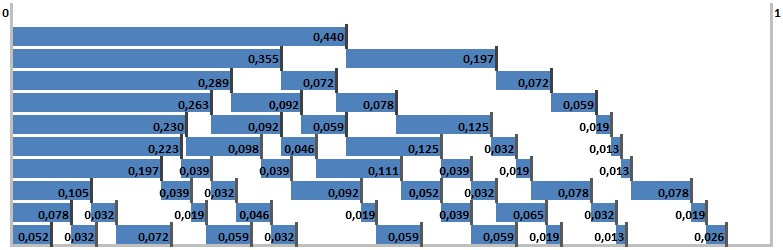
\includegraphics[scale=.7]{sections/images/consciousness_logical_moments.jpg}
\floatfoot{Exemplo de um intervalo lógico com dez momentos lógicos.}%\footnotemark}
\end{figure}
%\footnotetext{Fonte: note}

A consciência são os momentos lógicos de uma expansão representados em suas unidades.

\begin{figure}[H]
\caption{Intervalo lógico consciente}
\label{fig:consciousness}
\centering
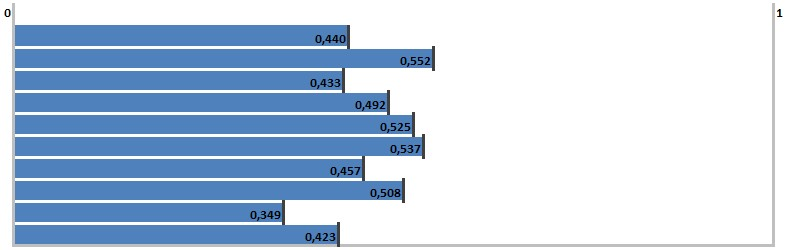
\includegraphics[scale=.7]{sections/images/consciousness.jpg}
\floatfoot{Exemplo de um intervalo lógico consciente com dez unidades de momentos lógicos.}%\footnotemark}
\end{figure}
%\footnotetext{Fonte: note}

Pode ser observado na Tabela \ref{tab:10000_all} que a probabilidade de 99,99\% das amostras, que aumentam em quantidade a medida que crescem os momentos lógicos, tendem a estar cada vez mais ao centro do intervalo lógico, sendo que essa centralização tende ao infinito.

\begin{figure}[H]
\caption{Centralização de 99,99\% das amostras}
\label{fig:centering_of_99_range}
\centering
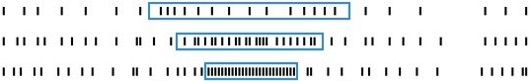
\includegraphics[scale=1]{sections/images/centering_of_99_range.jpg}
\floatfoot{Tendência de centralização do range de 99,99\% das amostras.}%\footnotemark}
\end{figure}
%\footnotetext{Fonte: note}

A consciência é o conjunto dos momentos lógicos unificados de uma expansão. É o aspecto da lógica que unifica as amostras desses momentos, ou seja, é a lógica que abstrai muitos em um, muitas subunidades em uma unidade por momento lógico. Todos os aspectos listados abaixo são inerentes a abstração da lógica chamada consciência.

\subsubsection{Infinito}
Um dos aspectos mais importantes que a negação do nada traz (negação de si), é o infinito, ou seja, em qualquer intervalo lógico cabe o infinito novamente. A lógica primordial que iniciou todo o intervalo lógico é a mesma encontrada em seus intervalos subsequentes. Isso fundamenta como uma lógica de alto nível como a consciência explica a lógica primordial, uma vez que não é preciso voltar ao primeiro momento lógico do intervalo para deduzi-lo, pois esse fenômeno é onipresente em todo o intervalo.

\subsubsection{Ondas}
Probabilisticamente a distribuição de novas amostras de uma população tendem a concentrar mais amostras sentido a mediana da população com frequências de amostras cada vez maiores neste sentido. Porém, a distribuição dessas amostras com frequências de crescimento uniformes é infinitesimal se comparado às possibilidades randômicas desse crescimento. Assim, a tendência de crescimento dessas frequências sentido a mediana somadas a baixíssima probabilidade (infinitesimal) desse crescimento ser uniforme, conduz a frequências no padrão de ondas.
\begin{figure}[H]
\caption{Padrão de onda}
\label{fig:consciousness_waves}
\centering
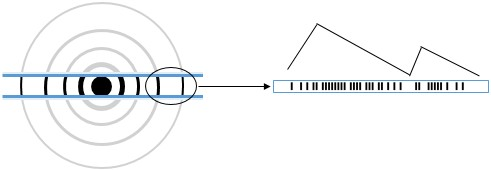
\includegraphics[scale=1]{sections/images/consciousness_waves.jpg}
\floatfoot{Padrão de onda inferido pela tendência dessa distribuição com frequências maiores sentido a mediana da população e a baixíssima probabilidade de crescimento uniforme dessas frequências.}%\footnotemark}
\end{figure}
%\footnotetext{Fonte: note}

Grandes intervalos com baixas frequências de amostras ou grandes intervalos com frequências uniformes de amostras são mais difíceis de observar devido à ausência de grandes discrepâncias. A junção de duas ondas além de eliminar suas discrepâncias, faz com que a primeira onda da união fique maior e a segunda onda acaba por deixar de existir e se tornar parte da primeira que tem seu pico mais próximo da mediana. Probabilisticamente uma onda não morre, apenas une-se com outras ondas mais internas a ela.
\begin{figure}[H]
\caption{Unificação de ondas}
\label{fig:consciousness_uniform_wave}
\centering
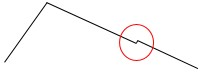
\includegraphics[scale=1]{sections/images/consciousness_uniform_wave.jpg}
\floatfoot{Ondas sendo unificadas para exemplificar o crescimento amostral uniforme.}%\footnotemark}
\end{figure}
%\footnotetext{Fonte: note}

\subsubsubsection{Entrelaçamento e subconsciente}
As amostras que mais se parecem em termos de frequências e distribuição são as amostras que fazem parte da mesma onda, que em momentos passados estiveram mais próximas. Elas são frequências opostas não sobrepostas que se completam.

Probabilisticamente as duas partes complementares de uma onda estarão a uma distância aproximadamente iguais, equidistante da mediana, porém essa não é uma regra e as partes complementares de uma onda podem estar em distâncias diferentes da mediana. O fenômeno da paridade das partes de uma onda tem o nome de entrelaçamento quântico.

Essas ondas formas subconsciência de uma consciência maior. A consciência é única para todo o intervalo, é a lógica do intervalo, enquanto forma subconsciências, como pequenas ondas de uma onda maior. Assim, uma mudança na onda maior (consciência) também é uma mudança na onda menor (subconsciência), mudança essa que é induzida pela subconsciência indiretamente, análogo ao comprimir gás em um cilindro, que ao adicionar uma nova molécula de gás no cilindro parcialmente cheio, mais próximas ou apertas as moléculas dentro dele estarão. O contrário também é verdadeiro, uma nova amostra em uma subconsciência, que por esta é observada diretamente é também uma mudança da consciência e vai ser induzida pelas outras subconsciências indiretamente.
\begin{figure}[H]
\caption{Subconsciência}
\label{fig:consciousness_subconscious}
\centering
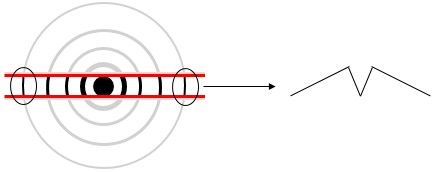
\includegraphics[scale=1]{sections/images/consciousness_subconscious.jpg}
\floatfoot{O padrão de ondas forma subconsciências semelhantes ao padrão criado pela consciência como visto na Figura \ref{fig:statisticsbyjim_central_limit_theorem} ou na Figura \ref{fig:trend_chart_of_normal_distribution}.}%\footnotemark}
\end{figure}
%\footnotetext{Fonte: note}

\subsubsection{Tempo}
O tempo é a adição de novos momento lógicos à medida que prossegue a negação desses momentos.  Essas mudanças são acumulativas e a medida que aumentam os número de amostras ou momentos lógicos, menos relevante cada nova amostra será dentro do intervalo consciente. Um em cem é mais relevante do que um em mil. 
\begin{figure}[H]
\caption{Tempo}
\label{fig:consciousness_time}
\centering
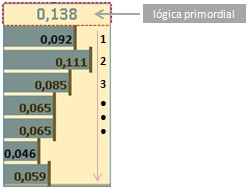
\includegraphics[scale=.8]{sections/images/consciousness_time.jpg}
\floatfoot{Progressão do tempo conforme os momentos lógicos avançam.}%\footnotemark}
\end{figure}
%\footnotetext{Fonte: note}

Outro fator importa a observar do tempo é que, probabilisticamente, subconsciências mais próximas da mediana da população terão uma adição maior de novas amostras em seus intervalos, o que são observados diretamente por essas subconsciências. Por outro lado, subconsciências distantes da mediana da população terão uma adição menor de amostras em seus intervalos e sujeitam-se a um número maior de mudança induzidas pela subconsciência indiretamente. Esse fenômeno de observação temporal proporcionado pela consciência e subconsciências evita o paradoxo dos gêmeos \cite{brasilescola_paradoxo_gemeos}.

Na seção Expansão binomial foi apresentado que a lógica é uma sequência de negações de si no tempo zero, ou seja, em nenhum momento entre suas negações a lógica passa a SER, garantindo a premissa primordial da constante lógica NÃO SER. Assim, a lógica é uma sequência infinita e simultânea, uma constante.
Logo, o tempo é apenas uma grandeza da consciência oriunda da sequência lógica. A simultaneidade dessa sequência torna a lógica uma constante com todas as suas infinitas possibilidades, sendo esse universo uma delas. Cada universo tem sua sequência de mudanças, que é estática, em uma ordem diferente e é essa ordem que dá origem à grandeza que chamamos de tempo. É essa ordem do universo ou consciência que vai dar a noção do que acontece antes ou depois, ou seja, o passado, o presente e o futuro.
Na experiência do tempo conduzida pela consciência a ordenação da sequência é a essência dessa grandeza e, portanto, mais relevante do que sua origem que é de natureza simultânea.

\subsubsection{Espaço}
As ondas da consciência exibidas em forma de histograma, onde as partes da onda que se completam são colocados lado a lodo é exibida na Figura \ref{fig:consciousness_space_waves}. 
\begin{figure}[H]
\caption{Histograma em padrão de ondas}
\label{fig:consciousness_space_waves}
\centering
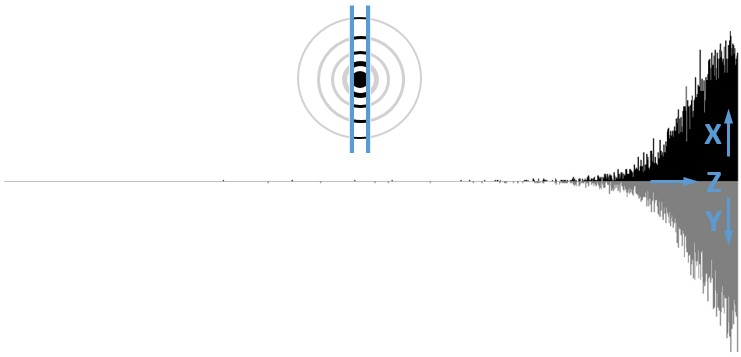
\includegraphics[scale=.7]{sections/images/consciousness_space_waves.jpg}
\floatfoot{Exemplo de padrão de ondas obtido pelo algoritmo Logic\_WavePattern \footnotemark.}
\end{figure}
\footnotetext{O algoritmo Logic\_WavePattern pode ser visto no Apêndice \ref{app:algoritmos}.}

Ao representar as grandezas espaciais conforme o gráfico a Figura \ref{fig:consciousness_space_waves} e distribuir seus pontos de extremidade (desprezando seus volumes e possíveis pontos internos) em um gráfico de distribuição 3D, obtém-se algo parecido com uma espiral (como redemoinhos no ar ou na água) mesmo em volumes muito pequenos de dados, conforme Figuras \ref{fig:consciousness_space_3DScatter15000-10} e \ref{fig:consciousness_space_3DScatter_200000-2}. Esses redemoinhos se movem lateralmente, uma vez que as coordenadas X e Y aumentam à medida que novas amostras são adicionadas na população. 
\begin{figure}[H]
\centering
	\begin{subfigure}[H]{0.47\linewidth}
	\centering
	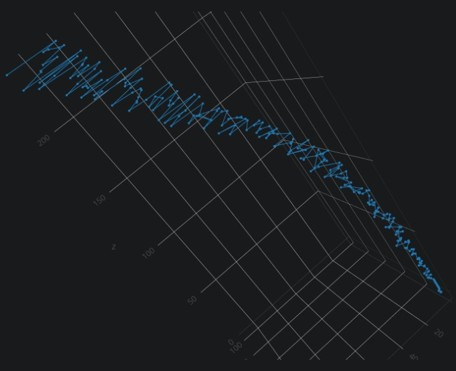
\includegraphics[width=.96\linewidth]{sections/images/consciousness_space_3DScatter15000-10.jpg}
	\caption{15.000 Amostras}
	\label{fig:consciousness_space_3DScatter15000-10}
	\end{subfigure}
\hfill
	\begin{subfigure}[H]{0.47\linewidth}
	\centering
	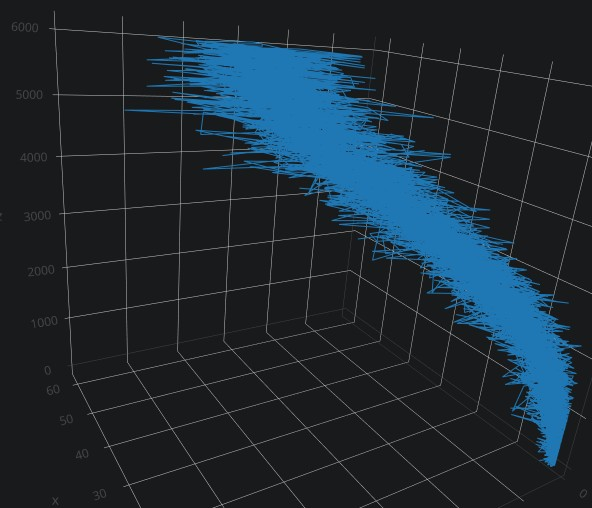
\includegraphics[width=.9\linewidth]{sections/images/consciousness_space_3DScatter_200000-2.jpg}
	\caption{200.000 Amostras}
	\label{fig:consciousness_space_3DScatter_200000-2}
	\end{subfigure}%
\caption{Gráfico de dispersão 3D gerado com os pontos do histograma em padrão de ondas}
\floatfoot{O histograma no padrão de ondas e os dados para gerar o gráfico de dispersão 3D podem ser obtidos com a execução do algoritimo Logic\_WavePattern \protect\footnotemark.}
\end{figure}
\footnotetext{O algoritmo Logic\_WavePattern pode ser visto no Apêndice \ref{app:algoritmos} e os gráficos de dispersão 3D podem ser acessados em: \url{https://chart-studio.plot.ly/create/?fid=ren.stuchi:5&fid=ren.stuchi:4} e \url{https://chart-studio.plot.ly/create/?fid=ren.stuchi:7&fid=ren.stuchi:6}}

A observação de outras subconsciências depende do range de ondas que uma subconsciência é capaz de observar e esse range, por sua vez depende do range de ondas que a própria subconsciência é constituída.

Em agrupamentos de amostras maiores pode-se ver o agrupamento de grandes objetos (subconsciências), sendo o maior deles representado pela cor azul claro e os menores e mais distantes pela cor azul escuro ou roxo, conforme Figura \ref{fig:consciousness_space_subconsciousness}. Esse agrupamento pode representar, por exemplo, o centro do universo, então o centro de uma galáxia, uma estrela, planetas e objetos menores e mais distantes.
\begin{figure}[H]
\caption{Abstração espacial das subconsciências - grande agrupamento de amostras}
\label{fig:consciousness_space_subconsciousness}
\centering
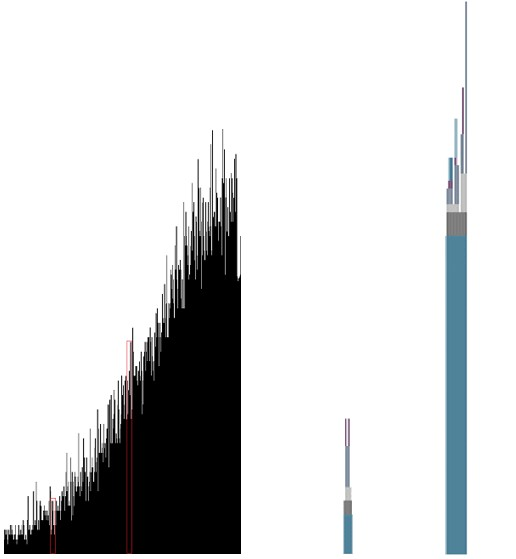
\includegraphics[scale=.5]{sections/images/consciousness_space_subconsciousness.jpg}
\floatfoot{Caracteristicas da ondas formadoras da subconsciência de grandes objetos.}%\footnotemark}
\end{figure}
%\footnotetext{Fonte: note}

Em agrupamentos de amostras menores pode-se ver o agrupamento de pequenos objetos (subconsciências). Quanto menores os agrupamentos menos divisões esses agrupamentos têm (cores), mais estreitos e compridos eles são, conforme Figura \ref{fig:consciousness_space_subconsciousness_min}. Esse agrupamento pode representar, por exemplo, o átomo que são muito pequenos, se apresentam em enormes quantidades e as partículas que orbitam seu núcleo ficam bem mais distantes dele.
\begin{figure}[H]
\caption{Abstração espacial das subconsciências - pequeno agrupamento de amostras}
\label{fig:consciousness_space_subconsciousness_min}
\centering

\includegraphics[scale=.9]{sections/images/consciousness_space_subconsciousness_min.jpg}
\floatfoot{Caracteristicas da ondas formadoras da subconsciência de pequenas partículas.}%\footnotemark}
\end{figure}
%\footnotetext{Fonte: note}}

Provavelmente, o padrão aproximado de espiral, visto nas Figuras \ref{fig:consciousness_space_3DScatter15000-10} e \ref{fig:consciousness_space_3DScatter_200000-2}, presentes também nas primeiras consciências (azul claro) refletirão nas subconsciências posteriores, pois estas são partes da primeira e assim por diante. Uma outra observação é que a consciência e suas subconsciências são uma mixagem dois eixos X com Y.

\subsubsubsection{Salto}
Em partículas muito pequenas como os elétrons pode-se notar o salto quântico (NUNES, 2019). O salto quântico é a incapacidade de uma determinada subconsciência observar subconsciência menores. Alguns equipamentos (sub-lógicas) podem melhorar essas observações, se aprofundando em detalhes e visualizando agrupamentos de amostras ainda menores e menores até que talvez se possa visualizar uma única amostra, conforme Figura \ref{fig:consciousness_space_subconscious_observation}. 

Outro fator que impacta para a observação desse salto é que as amostras de um intervalo podem negar esse intervalo de diferentes formas ou valores, assim a representação desses valores nas barras do histograma (que representa os eixos X e Y) devem corresponderem a esses valores, o que fará com que os valores da barra X ou Y sejam incrementados com valores superiores a um, frequentemente. A representação das barras do histograma é a soma das amostras, com um fatorial. Assim um intervalo que contenha as amostras 1, 2 e 3 será represento com uma barra de valor 6, ao invés de incrementos de 1 em 1 o que daria o valor 3 para essa barra, conforme Figura \ref{fig:consciousness_space_subconscious_observation_jump}. Ou seja, a mesma quantidade de amostras de um intervalo podem produzir diferentes posições espaciais que condizem a esses valores. 
\begin{figure}[H]
\centering
	\begin{subfigure}[H]{0.8\linewidth}
	\centering
	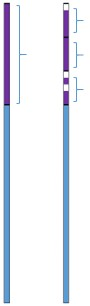
\includegraphics[width=.2\linewidth]{sections/images/consciousness_space_subconscious_observation.jpg}
	\caption{}
	\label{fig:consciousness_space_subconscious_observation}
	\end{subfigure}
\hfill
	\begin{subfigure}[H]{0.8\linewidth}
	\centering
	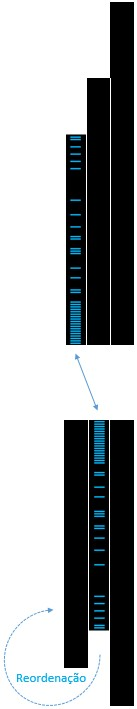
\includegraphics[width=.9\linewidth]{sections/images/consciousness_space_subconscious_observation_jump.jpg}
	\caption{}
	\label{fig:consciousness_space_subconscious_observation_jump}
	\end{subfigure}%
\caption{Observações subconscientes}
\floatfoot{Diferentes subconsciências diferentes observações dos intervalos de ondas..} %\protect\footnotemark.}
\end{figure}
%\footnotetext{}

\subsubsection{Forças fundamentais}
A força gravitacional, a força eletromagnética e a força nuclear correspondem às forças fundamentais da natureza e essas forças são provenientes do entrelaçamento quântico:

\subsubsubsection{Força gravitacional}
O entrelaçamento quântico, que define os pares de ondas opostas não sobrepostas que se completam e que mais se assemelham em termos de frequência e distribuição das amostras, é o aspecto que coordena as mudanças nas coordenadas espaciais X, Y e Z. As mudanças dessas coordenadas provocam iterações que podem ser vistas nas Figuras \ref{fig:consciousness_space_3DScatter15000-10} e \ref{fig:consciousness_space_3DScatter_200000-2} da subseção de Espaço. Essas iterações têm o nome de gravidade.

\subsubsubsection{Força eletromagnética}
A força eletromagnética é uma especificação da força gravitacional que depende da aproximação espacial (redução de diferenças nos eixos X, Y e Z) e do entrelaçamento quântico estabelecido pela gravidade.

Quando um objeto se aproxima de outro, seus pares de ondas provenientes do entrelaçamento quântico ficam cada vez mais parecidos, eixos X e Y. Essa proximidade faz com partes de ondas de um objeto se pareça muito com as partes da onda do outro objeto, o que pode fazer com que o entrelaçamento quântico encontre pares mais ideais nesse outro objeto e vice-versa.  

As linhas azuis da Figura \ref{fig:consciousness_electromaagnetic_force} mostra onde é mais frequente a troca dos pares de ondas pelo entrelaçamento quântico, ou seja, a probabilidade maior das ondas serem parecidas. Por isso os imãs tentam se virar para se conectar quando estão face a face com lados iguais. As linhas cinza mostram as conexões que ocorrem um número menor. 
\begin{figure}[H]
\caption{Força eletromagnética}
\label{fig:consciousness_electromaagnetic_force}
\centering
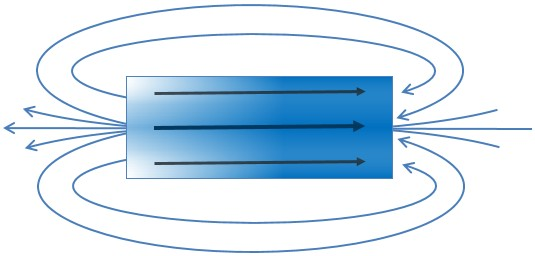
\includegraphics[scale=.8]{sections/images/consciousness_electromaagnetic_force.jpg}
\floatfoot{Aumento das possibilidades de entrelaçamento quântico devida a aproximação e menor número de amostras das menores partículas. }%\footnotemark}
\end{figure}
%\footnotetext{Fonte: note}

Quanto menor a partícula (elétron ou partículas menores), conforme Figura \ref{fig:consciousness_space_subconsciousness_min}, mais fácil o entrelaçamento ocorre. Provavelmente muitos objetos não tenham alta capacidade de entrelaçamento devido aos seus elétrons ou partículas menores serem formadas por muitas amostras (barras do histograma mais largas ou mais compridas), ou seja, quanto maior a quantidade de amostras dessas partículas menores as chances de entrelaçamento. 

Probabilisticamente as partículas mais parecidas estão nas regiões mais próximas (linhas azuis do Figura \ref{fig:consciousness_electromaagnetic_force}), porém isso não é uma regra e um polo podem se inverter, ou seja, ter mais ligações com a região de menor probabilidade (isso não quer dizer que houve formação de antimatéria nos átomos dessa região). No entanto, a probabilidade tende a corrigir esse polo conforme novas amostras vão sendo adicionadas nesse intervalo. 


\subsubsubsection{força nuclear}
As forças nucleares forte e fraca representam as maiores concentrações de amostras por intervalo populacional. Esses picos de amostras podem ser vistos na Figura \ref{fig:consciousness_space_subconsciousness_min} e esses picos não para de crescer à medida que novas amostras deixam ainda mais apertada essa proporção de intervalo e amostras, uma vez que essas amostras tendem a estarem cada vez mais juntas.

\subsubsection{Matéria escura e energia escura}
Quanto maior o número de amostras e mais próximas elas estão da mediana, mais elas farão parte dos 99,99\% e ainda mais amostras também estarão nos 0,01\%, conforme a Tabela \ref{tab:10000_all}. Assim, a observação desses 0,01\% passa a ser cada vez mais difícil, pois sua relevância consciente passa a ser cada vez mais próxima de zero. É importante notar também que a medida que os 99,99\% aumentam em número de amostras, menos relevante cada nova amostra será dentro desse conjunto (um em cem é mais relevante do que um em mil) e uma porcentagem menor será ocupada pelo range dos 99,99\% das amostras, conforme a Tabela \ref{tab:10000_all}.

\begin{figure}[H]
\caption{Analogia da matéria escura e energia escura}
\label{fig:consciousness_dark_matter_dark_energy}
\centering
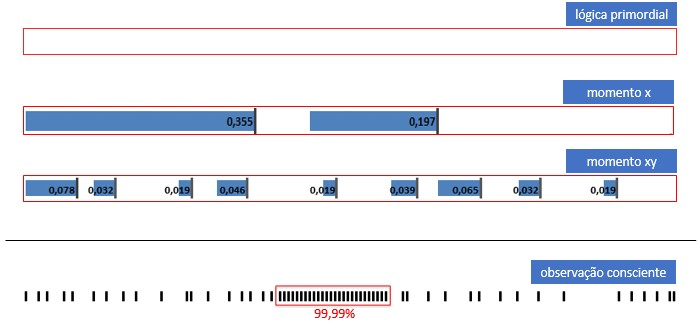
\includegraphics[scale=1]{sections/images/consciousness_dark_matter_dark_energy.jpg}
\floatfoot{Fenômenos antevistos ou conjecturados pela consciência.}%\footnotemark}
\end{figure}
%\footnotetext{Fonte: note}

\subsubsection{Antimatéria}
Independente do intervalo observado (análogo à bytes, kilobytes, prótons, elétrons etc.), que são contextos lógicos de observação e/ou utilização consciente, este pode estar com sua maior concentração de amostras no sentido da mediana, o que é o sentido provável conforme os números de amostras crescem em um intervalo, conforme teorema central do limite. Essas amostras também podem estar com sua concentração no sentido oposto a mediana, porém com uma ocorrência probabilística cada vez menos conforme as amostras aumentam. Na Figura \ref{fig:consciousness_concentration_of_opposite_samples} é exibido dois intervalos idênticos com suas amostras com concentrações opostas.

\begin{figure}[H]
\caption{Parte de um intervalo idêntico com suas concentrações de amostras opostas}
\label{fig:consciousness_concentration_of_opposite_samples}
\centering
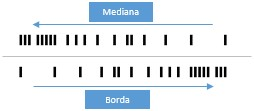
\includegraphics[scale=1]{sections/images/consciousness_concentration_of_opposite_samples.jpg}
\floatfoot{Parte de um intervalo idêntico distribuídos de formas opostas.}%\footnotemark}
\end{figure}
%\footnotetext{Fonte: note}

O merge ou soma dos intervalos opostos da Figura \ref{fig:consciousness_concentration_of_opposite_samples} os tornaria um intervalo simétrico, ou seja, não estaria em nenhum dos sentidos.
Na Figura \ref{fig:consciousness_concentration_of_opposite_samples_within_range} é exibido um intervalo consciente completo com suas concentrações de amostras sentido à mediana e outro idêntico, mas com suas concentrações sentido às bordas do intervalo.

\begin{figure}[H]
\caption{Intervalos conscientes com suas concentrações de amostras opostas}
\label{fig:consciousness_concentration_of_opposite_samples_within_range}
\centering
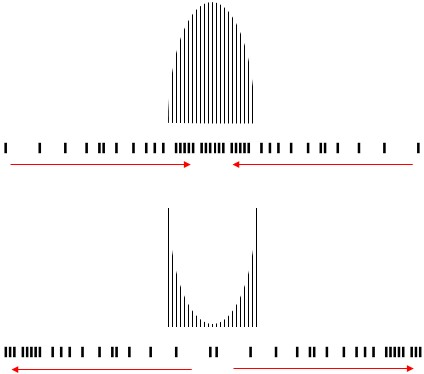
\includegraphics[scale=.8]{sections/images/consciousness_concentration_of_opposite_samples_within_range.jpg}
\floatfoot{Intervalos conscientes completos e idênticos distribuídos de formas opostas.}%\footnotemark}
\end{figure}
%\footnotetext{Fonte: note}


\subsubsection{Buraco negro}
O buraco negro é uma concentração muito alta de amostras, formada por grandes agrupamentos subconscientes, Figura \ref{fig:consciousness_space_subconsciousness}.
Esses grandes agrupamentos ocupam grandes volumes de espaço devido a quantidade de amostras, porém suas ondas têm baixas discrepância o que os torna menos observáveis. 

Os grandes volumes são encontrados na base dos grandes agrupamentos, conforme as cores azul claro e cinza da Figura \ref{fig:consciousness_black_hole}.
\begin{figure}[H]
\caption{Buracos negros}
\label{fig:consciousness_black_hole}
\centering
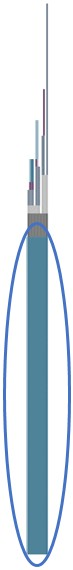
\includegraphics[scale=.6]{sections/images/consciousness_black_hole.jpg}
\floatfoot{Grandes volumes são encontrados na base dos grandes agrupamentos.}%\footnotemark}
\end{figure}
%\footnotetext{Fonte: note}